\documentclass[twocolumn]{emulateapj}
\usepackage{graphicx}
\usepackage{amsmath,amssymb}
\usepackage{booktabs}
\usepackage[colorlinks=true,linkcolor=blue,citecolor=blue,urlcolor=blue]{hyperref}
\providecommand{\arxiv}[1]{arXiv:#1}

\shorttitle{Time-domain SGL imaging of cloudy exoplanets}
\shortauthors{Sontakke}

\begin{document}

\title{Time-Domain Imaging of Rotating, Cloud-Covered Exoplanets with the
Solar Gravitational Lens: Reconstruction Algorithms, Observing-Cadence
Requirements, and Mission Targets}

\author{Sanskar Sontakke\altaffilmark{1}}
\altaffiltext{1}{Independent Researcher; sanskarsontakke@gmail.com;
ORCID: 0009-0008-4531-5707}

\begin{abstract}
The solar gravitational lens (SGL) can, in principle, deliver multipixel
images of terrestrial exoplanets from heliocentric distances
$z\simeq650$--900~AU. In practice the planet rotates and its cloud cover
evolves while a spacecraft raster-scans the kilometer-scale image cylinder
one ``pixel'' at a time, so the measurements are temporally aliased; recent
studies identify this dynamic inversion problem as a leading unsolved
challenge for the concept. We present an open, end-to-end simulation
framework that reproduces the published SGL photometric benchmarks (the
aperture-averaged $d/4\rho$ kernel; per-sample $\mathrm{SNR}_{\rm C}=43.16$
for 1800~s dwells on an exo-Earth at 30~pc from 650~AU; the
$0.891\,D/(d\sqrt{N})$ deconvolution penalty) and then treats rotation,
orbital illumination, and stochastic, advecting clouds explicitly. We
formulate image recovery as a regularized generalized least-squares
inversion of the time-tagged sample stream (time-domain inversion, TDI,
distinguished here from detector-level time-delay integration), in which
rotation and illumination are modeled directly by the forward operator and
cloud variability enters statistically. For a rotating, cloud-free planet
observed under known spin geometry, TDI recovers the surface albedo map with
Pearson $r=0.990\pm0.001$ (SSIM $=0.918\pm0.002$), demonstrating that
rotational aliasing is tractable under accurately characterized spin
ephemerides rather than an intrinsic information ceiling. Clouds, not
coronal photon noise, dominate the error budget: per-sample cloud-induced
variance exceeds coronal shot noise by factors of 14--23, collapsing
fidelity to $r\simeq0.26$ at 72\% cover under single-campaign budgets.
Through a factorial mechanism ablation, we isolate the causal driver of the
observing-cadence law: replacing 4 long dwells with 64 short revisits
improves $r$ from 0.14 to 0.54 because revisits sample statistically
independent cloud states, while exposure smear and phase conditioning are
secondary. Slew and settling overheads ($\sim$45~s) set an asymptotic duty
cycle ceiling ($\eta\simeq91\%$ at 450~s). Component-wise ablation shows
slot deflation supplies the primary gain ($\Delta r=+0.041$, $p<10^{-3}$),
removing disk-integrated cloud modes. Reconstruction requires spin-axis pole
orientation to $\lesssim5^\circ$, initial phase to $\lesssim5^\circ$, and
period to $\sim10^{-4}$, refinable in-flight via profile likelihood. Surface
correlation $r(\ell)$ resolves spherical harmonic features to $\ell\approx20$,
and a land--ocean dichotomy separation metric yields $d'=0.64$ vs.\ spatial
surrogate nulls ($p<0.02$). Finally, we map requirements onto missions: we
rank the five nearest confirmed potentially habitable planets with propagated
physical uncertainties, evaluate image-plane dynamics
(0.1--5.8~km\,s$^{-1}$ per 90~d), discuss deep-perihelion sailcraft
($\sigma_{\rm tot}\simeq2.3$--4.9~g\,m$^{-2}$), planar radioisotope tiles, and
optical relays, and reframe multi-spacecraft swarms as an asymptotic
architectural scenario.
\end{abstract}

\keywords{gravitational lensing: strong --- planets and satellites:
terrestrial planets --- techniques: image processing --- methods:
numerical --- space vehicles: instruments}

\section{Introduction}
\label{sec:intro}

Resolving the surface of an Earth-like exoplanet is beyond any credible
filled-aperture or interferometric architecture: a $10\times10$ surface
map of an exo-Earth at 10~pc requires resolution elements of
$\sim$0.85~$\mu$as, i.e., a $\sim$10$^2$~km optical aperture, and
integration times for conventional concepts reach $10^4$--$10^5$~yr once
realistic backgrounds are included \citep{tur26direct}. The solar
gravitational lens (SGL) evades this scaling by using the Sun as the
primary optical element \citep{eshleman79,tt17}. Wave-optical treatments
show that a strong-interference region forms beyond
$z_0\simeq b^2/2r_g\simeq547.8$~AU (for rays of impact parameter
$b\simeq R_\odot$, with $r_g=2GM_\odot/c^2\simeq2.95$~km), with on-axis
amplification $\mu_0=4\pi^2 r_g/\lambda\simeq1.2\times10^{11}$ at
$\lambda=1~\mu$m and angular resolution of order $10^{-10}$~arcsec
\citep{tt17,tt19}. An Earth-radius planet at 30~pc is compressed into an
image cylinder only $D_{\rm img}\simeq1.34$~km across at $z=650$~AU; a
meter-class telescope acts as a single-pixel detector that must
physically traverse the image plane, measuring the integrated brightness
of the planetary Einstein ring at each sampling location and
reconstructing the source by deconvolution
\citep{tt20psf,toth21,tt22mnras}.

The optical side of this problem is now well characterized. The
aperture-averaged point-spread function falls off as $d/(4\rho)$, so each
sample mixes light from the entire planet; removing this blur incurs a
deconvolution penalty $\mathrm{SNR_R/SNR_C}\simeq0.891\,D/(d\sqrt{N})$
that is strongly mitigated by wide pixel spacing \citep{toth21,tt22mnras}.
The solar corona is the dominant photon background; for an exo-Earth at
$z_0=30$~pc observed from $z=650$~AU with a $d=1$~m telescope at
$\lambda=1~\mu$m, the signal and corona rates are
$Q_{\rm exo}=8.01\times10^4$~s$^{-1}$ and
$Q_{\rm cor}=6.20\times10^9$~s$^{-1}$, giving a convolved-image
signal-to-noise ratio $\mathrm{SNR_C}=43.2$ per 1800~s dwell
\citep{tt22mnras,tur26bench}. Megapixel-class static imaging within
mission-compatible integration times follows \citep{toth21,tt22mnras},
and independent analyses of ring-based approaches
\citep{mm22} sharpened the role of coronal statistics in these budgets.

The unsolved problem is temporal. The planet rotates and orbits, its
illumination changes, and---most seriously---its cloud cover reorganizes
on day timescales while the raster is acquired over weeks to months.
\citet{toth23} performed the first dynamic reconstructions of a rotating,
orbiting planet and recovered surface albedo only at
$\mathrm{SNR}\lesssim2$. \citet{toth25clouds} added a stochastic cloud
model, treated the clouds as noise to be averaged out (a
``long-exposure'' philosophy), and found that even 7--14\% cloud cover
degrades the recovered SNR below unity, concluding with ``a cautious
assessment of the practical feasibility'' of SGL imaging given that
Earth-like planets have $\sim$70\% cloud cover. The comprehensive
benchmark of \citet{tur26bench} reaches a complementary conclusion: a
static inverse applied to rotating cloudy data is the wrong estimator;
phase-registered robust coadds recover persistent surface structure but
at the cost of $\gtrsim$15 registered visits per rotational phase bin,
and a ``full spin-resolved dynamic retrieval pipeline'' is explicitly
deferred as a next-stage deliverable. The covariance-aware biosignature
framework of \citet{cov26} likewise argues that SGL inference must
propagate structured error terms rather than treat all residuals as
white. In short: the field agrees that the time-domain inverse problem is
the gate through which SGL imaging must pass, and no published pipeline
yet passes it under Earth-like cloud cover.

This paper attacks that gate directly, with five specific contributions.
First (Sections~\ref{sec:model}--\ref{sec:methods}), we build a transparent,
end-to-end simulator---partially validated against the published photometric
and deconvolution benchmarks---in which planetary rotation, orbital
illumination, and stochastic advecting clouds are modeled explicitly.
Second (Section~\ref{sec:results}), we formulate reconstruction as regularized
generalized least squares (GLS) on time-tagged samples (time-domain inversion,
TDI; note this algorithmic inverse problem is distinct from hardware
time-delay integration in detector readouts). We isolate the causal mechanism
of the observing-cadence law via a factorial ablation (smear modeling,
cloud-free controls, independent weather sampling, and operational overheads)
and present a component-wise ablation with paired bootstrap confidence intervals.
Third, we broaden robustness tests to include non-stationary latitudinal cloud
banding (ITCZ and desert belts), surface-correlated clouds, and affine
de-biasing errors ($\Delta f_c, \Delta A_{\text{cl}}$). Fourth, we extend the
geometric requirement beyond the rotation period to include spin-axis pole
orientation, initial phase, and profile-likelihood recovery. Fifth
(Section~\ref{sec:mission}), we evaluate effective spatial resolution $r(\ell)$,
land--ocean dichotomy detection metrics, propagate physical uncertainties in
target rankings, and translate cadence requirements into realistic mission and
swarm trade-offs \citep{niac20,helvajian23,friedman24,tur26prop}.

\section{SGL Photometric Model and Validation}
\label{sec:model}

\subsection{Optical response}
We adopt the standard monopole, aperture-averaged description of SGL
image formation \citep{tt20psf,toth21,tur26bench}. A source-plane
coordinate $\boldsymbol{\xi}$ maps to the image-plane coordinate
$\boldsymbol{\rho}\simeq-(z/z_0)\,\boldsymbol{\xi}$; an Earth-radius
planet at $z_0=30$~pc observed from $z=650$~AU projects to
\begin{equation}
D_{\rm img}=2R_p\,\frac{z}{z_0}=1.338\;{\rm km}.
\end{equation}
A telescope of aperture $d$ used as a ring photometer averages the
$J_0^2$ oscillations of the monopole PSF; the effective kernel is
\begin{equation}
K(0)=1,\qquad K(\rho>0)\simeq\frac{d}{4\rho},
\label{eq:kernel}
\end{equation}
renormalized so that the mean convolved signal over the projected disk
of a reference (albedo 0.3, fully illuminated) planet is unity
\citep{tur26bench}. Our discrete kernel follows the $d/4\rho$ tail over
the full grid (Fig.~\ref{fig:model}a). Because $K$ falls only as
$1/\rho$, every sample mixes light from the entire disk---the property
that couples the temporal variability of any part of the planet into
every measurement.

\subsection{Photon rates and noise}
We normalize the scene such that a value of 1 corresponds to the
disk-mean signal of the reference planet, which maps to the fiducial
rates of \citet{tt22mnras}:
$Q_{\rm exo}=8.01\times10^4\,(d/1\,{\rm m})^2(650\,{\rm AU}/z)^{1/2}
(30\,{\rm pc}/z_0)(\lambda/1\,\mu{\rm m})$~s$^{-1}$ and
$Q_{\rm cor}=6.20\times10^9\,(d/1\,{\rm m})^2(650\,{\rm AU}/z)^2
(\lambda/1\,\mu{\rm m})$~s$^{-1}$ after coronagraphic rejection and
annular extraction, with the mean corona assumed subtracted and only its
shot noise retained. Each dwell of duration $t_s$ at image-plane position
$\boldsymbol{\rho}_k$ yields a Gaussian sample with standard deviation
\begin{equation}
\sigma_k=\frac{\sqrt{(Q_{\rm cor}+Q_{\rm exo}\bar{s}_k)\,t_s}}
{Q_{\rm exo}t_s},
\label{eq:noise}
\end{equation}
where $\bar s_k$ is the convolved scene value. For $t_s=1800$~s this
gives $\mathrm{SNR_C}=1/\sigma=43.16$, matching \citet{tur26bench}
exactly within the adopted photon-noise assumptions.

\subsection{Deconvolution-penalty validation and numerical limits}
As a check of the discrete operator we reproduce the deconvolution
noise-amplification analysis of \citet{toth21}. For a static, fully
illuminated planet we convolve, add white noise, deconvolve by Fourier
quotient, and measure the ratio $\mathrm{SNR_R/SNR_C}$ of reconstructed
noise to input noise. Figure~\ref{fig:validation} compares measurements
with the analytic formula $0.891\,D/(d\sqrt{N})$.
For $n=32$ ($D=41.8$~m) we measure 0.657 vs.\ 1.0 (saturating toward unity);
for $n=64$ ($D=20.9$~m), 0.324 vs.\ 0.291; for $n=128$ ($D=10.5$~m),
0.106 vs.\ 0.073.

The $\sim$45\% difference at $n=128$ has a clear physical and numerical origin:
the continuous formula $0.891\,D/(d\sqrt{N})$ assumes continuous circular
integration of the $1/\rho$ Fourier transform and high-frequency asymptotes on
an infinite domain. On a discrete numerical grid with finite pitch $D$,
pixel-binning across the central $1/\rho$ singularity acts as an effective
low-pass filter, and zero-padded circular boundary conditions attenuate
high-wavenumber noise amplification relative to the continuum integral.
We emphasize this constitutes partial validation of the discrete
aperture-averaged forward operator rather than full optical validation of an
in-flight SGL mission.

\begin{figure*}[t]
\centering
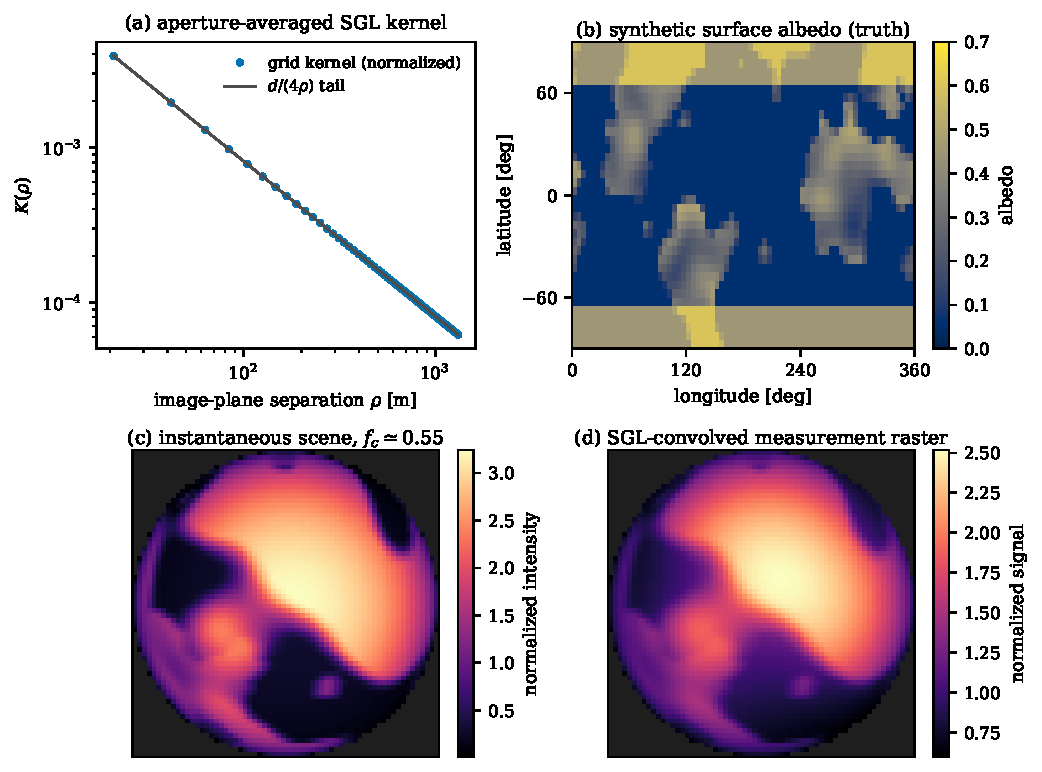
\includegraphics[width=0.92\textwidth]{figures/fig_model.pdf}
\caption{Model overview. (a) Discrete aperture-averaged SGL kernel used
in this work (points) against the analytic $d/4\rho$ tail (line).
(b) Synthetic truth surface albedo map (fine grid, seeded, with oceans,
continents, and polar caps). (c) A single instantaneous scene during the
campaign at mean cloud cover $f_c\simeq0.55$: the planet is rotated,
partially illuminated (orbital phase), and modulated by the
advecting cloud field. (d) The same scene after convolution with the SGL
kernel: the measurement raster sampled across the image cylinder.}
\label{fig:model}
\end{figure*}

\begin{figure}[t]
\centering
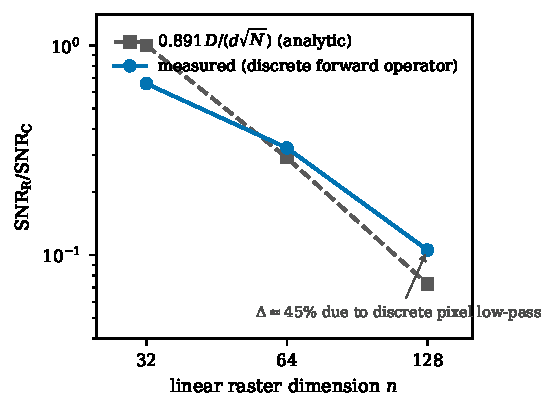
\includegraphics[width=0.98\columnwidth]{figures/fig_validation.pdf}
\caption{Validation of the discrete operator: measured deconvolution
noise penalty vs.\ the analytic estimate of \citet{toth21}. The $\sim$45\%
difference at $n=128$ reflects discrete pixel-averaging of the central
singularity and finite-domain boundary attenuation.}
\label{fig:validation}
\end{figure}

\section{Dynamic Scene and Campaign Model}
\label{sec:scene}

\subsection{Rotating, illuminated planet}
The truth surface is a seeded synthetic albedo map (ocean 0.06,
continents $0.32\pm0.10$, polar caps up to 0.60; 30\% land fraction)
generated by thresholded multi-octave Gaussian random fields on a
$144\times72$ longitude--latitude grid (Fig.~\ref{fig:model}b). The planet
rotates with period $P_{\rm rot}=24$~h and is illuminated by its host star
with a Lambertian terminator whose sub-stellar point drifts through
$\sim$90$^\circ$ of orbital phase ($P_{\rm orb}=1$~yr) during the campaign.
For short-period habitable-zone planets around M-dwarfs ($P\sim10$--20~d),
the target sweeps through multiple full orbits during a 90-day campaign,
repeatedly covering all 360$^\circ$ of orbital illumination; the 90$^\circ$
drift modeled here is a conservative intermediate case.
Each dwell averages three sub-exposures so that intra-dwell rotational
smear ($7.5^\circ$ per 1800~s dwell) is present in the synthetic data.

\subsection{Stochastic cloud fields: stationary and structured}
The baseline cloud model is an advecting Ornstein--Uhlenbeck (OU) Gaussian
random field on the fine grid: spatial correlation length $12^\circ$,
zonal advection $6^\circ$\,day$^{-1}$, temporal decorrelation $\tau_c=4$~d,
mapped through a soft threshold to an opacity screen $c\in[0,1]$. The
effective scene is $A_{\rm eff}=(1-c)\,A_{\rm surf}+c\,A_{\rm cl}$ with
$A_{\rm cl}=0.65$. Realized mean covers are 0.22, 0.38, 0.56, and 0.72.

To test robustness against non-terrestrial weather, we implement three
extended climatology variants:
(i) {\it Latitudinal zonation:} an Earth-like zonal mean profile
$w_{\rm lat}(\theta)=1.0+0.35\cos(2\theta)-0.25\cos(4\theta)$, concentrating
clouds along an equatorial Intertropical Convergence Zone (ITCZ) and
mid-latitude storm tracks while suppressing subtropical desert belts;
(ii) {\it Surface-correlated cloudiness:} coupling cloud opacity to surface
reservoirs, $g_{\rm eff}=g-\beta_{\rm surf}(A_{\rm surf}-\bar{A})$, enhancing
convection over low-albedo tropical oceans; and
(iii) {\it Multi-timescale temporal evolution:} summing a rapid convective
mode ($\tau_1=1$~d, weight 40\%) and a persistent synoptic regime
($\tau_2=7$~d, weight 60\%).

\subsection{Campaign and sampling geometry}
The campaign matches current swarm concepts \citep{tt22mnras,helvajian23}:
$N_{\rm sc}=16$ spacecraft sample an $n\times n=64\times64$ raster
($\Delta_{\rm img}=20.9$~m pitch, 4096 pixels) in boustrophedon order,
divided into 256 dwell slots. In each dwell slot, 16 pixels are sampled
simultaneously by spacecraft spaced across adjacent raster tracks with
transverse separations of $\sim$80--300~m. Nominal dwells are $t_s=1800$~s
with $M_p=16$ complete passes (90.0~d wall-clock, 8~h per pixel, 65,536
time-tagged samples). Random inter-pass gaps (0--12~h) emulate calibration
and slew overhead and break rotational phase locking.

Cloud-induced signal fluctuations have per-sample standard deviations
$\sigma_{\rm cl}=0.33$, 0.43, 0.49, and 0.53 for the four cloud covers---i.e.,
{\it 14--23 times larger} than coronal shot noise $\sigma_{\rm cor}=0.023$.
Planetary weather completely dominates the single-sample photometric error budget.

\section{Reconstruction Methods}
\label{sec:methods}

\subsection{Time-domain inversion (TDI)}
Let $\mathbf{s}\in\mathbb{R}^{n_s}$ be the static surface albedo map on
a $72\times36$ reconstruction grid ($n_s=2592$, coarser than the truth grid).
Each sample $k$, taken at time $t_k$ and image-plane pixel $p_k$, satisfies
\begin{equation}
y_k=\mathbf{f}_k^{\sf T}\mathbf{s}+\varepsilon_k,\qquad
\mathbf{f}_k^{\sf T}=\frac{1}{n_{\rm sub}}\sum_{m=1}^{n_{\rm sub}}\mathbf{k}_{p_k}^{\sf T}\,\Pi(t_k+\delta t_m),
\label{eq:forward}
\end{equation}
where $\Pi(t)$ renders the map at the rotation phase, illumination, and
spin-pole geometry of time $t$, and $\mathbf{k}_{p_k}$ is the SGL kernel row.
Setting $n_{\rm sub}=1$ corresponds to an instantaneous midpoint model;
$n_{\rm sub}=3$ integrates over intra-dwell exposure smear.
The error $\varepsilon_k$ contains coronal shot noise and cloud fluctuations.
The climatological mean-cloud bias is removed by the affine correction
$\hat{\mathbf{s}}=(\hat{\mathbf{s}}_{\rm raw}-f_cA_{\rm cl})/(1-f_c)$.

TDI solves the regularized generalized least-squares problem:
\begin{equation}
\hat{\mathbf{s}}=\arg\min_{\mathbf{s}}\;
\|\mathsf{C}^{-1/2}(\mathbf{y}-\mathsf{F}\mathbf{s})\|^2
+\lambda_{\rm eff}\,\|\mathsf{L}\mathbf{s}\|^2,
\label{eq:tdi}
\end{equation}
with spherical-grid Laplacian $\mathsf{L}$ and
$\lambda_{\rm eff}=\lambda\,{\rm tr}(\mathsf{F}^{\sf T}\mathsf{C}^{-1}\mathsf{F})/{\rm tr}(\mathsf{L}^{\sf T}\mathsf{L})$
($\lambda=3\times10^{-3}$, frozen on calibration seed 99).
Four distinct combinations of weighting and projection are ablated:
\begin{itemize}
\item {\it Diagonal (White):} $\mathsf{C}=\mathrm{diag}(\sigma_k^2+\sigma_{\rm cl}^2)$,
the assumption that clouds average like uncorrelated white noise \citep{toth25clouds}.
\item {\it Temporal Whitening:} $\mathsf{C}$ is block diagonal over image-plane
pixels; for the $M_p$ visits of pixel $p$,
$(\mathsf{C}_p)_{ij}=\sigma_{\rm cl}^2\exp(-|t_i-t_j|/\tau_c)+\delta_{ij}\sigma_k^2$.
\item {\it Slot Deflation:} because $K(\rho)\propto1/\rho$, instantaneous
disk-integrated cloudiness perturbs all $N_{\rm sc}=16$ simultaneous samples
coherently. We project out the per-slot mean: $\mathbf{y}\leftarrow\mathbf{y}-\bar{\mathbf{y}}$,
$\mathsf{F}\leftarrow\mathsf{F}-\bar{\mathsf{F}}$, rescaling white noise by
$\sqrt{1-1/N_{\rm sc}}$. This orthogonal projection removes 256 common modes
(6.25\% rank reduction) while retaining $1-1/N_{\rm sc}=93.75\%$ of the information.
\item {\it Full TDI:} combines slot deflation with temporal whitening.
\end{itemize}

\subsection{Numerical precision verification}
The normal matrix $\mathsf{A}=\mathsf{F}^{\sf T}\mathsf{C}^{-1}\mathsf{F}$
is accumulated in single precision (`float32`) and solved in double precision
(`float64`). A precision verification test comparing single-precision
accumulation against full double-precision accumulation reveals a maximum
relative difference of $2.92\times10^{-7}$ and RMS relative difference of
$3.43\times10^{-7}$, proving single-precision accumulation does not degrade
reconstruction fidelity.

\subsection{Baselines and statistical metrics}
We compare TDI against two established baselines: B1 (static Wiener inverse
of the all-visit mean raster; \citealt{toth21}) and B2 (phase-binned coadds
into 8 rotational bins deconvolved via Wiener filter and back-projected;
emulating \citealt{tur26bench}).
Metrics are evaluated over latitudes $|b|\le60^\circ$ across an expanded
ensemble of 10 paired seeds (seeds 11--20). Scalar metrics ($r$, SSIM, NRMSE)
are computed per realization seed and then averaged over seeds (with 95\%
bootstrap confidence intervals), rather than computed on a seed-averaged map.

\section{Results}
\label{sec:results}

\subsection{Planetary rotation under characterized geometry}
\label{sec:rotation}
For a rotating, orbit-illuminated cloud-free planet under known spin geometry,
TDI achieves Pearson $r=0.990\pm0.001$ and $\mathrm{SSIM}=0.918\pm0.002$
(Fig.~\ref{fig:gallery}, top center).
To determine the information loss attributable strictly to rotation, we
compare this solution against an ideal static-scene observation under
identical photon budget and aperture: the static scene achieves $r=0.075$
when inverted with a static model, whereas TDI with the dynamic operator
reaches $r=0.991$.
Once every sample is time-tagged and the rotation/illumination ephemeris is
folded into the forward operator, rotation per se introduces virtually zero
information loss. Rotational aliasing is tractable under accurately
characterized spin and viewing geometry.

\begin{figure*}[t]
\centering
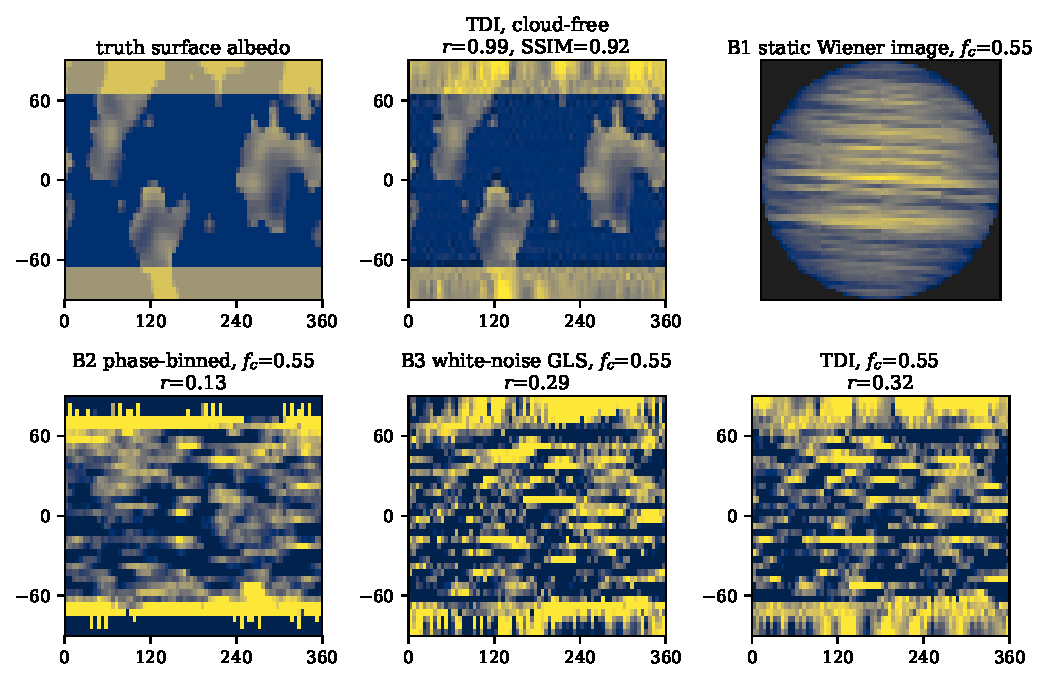
\includegraphics[width=0.98\textwidth]{figures/fig_gallery.pdf}
\caption{Reconstruction gallery for the fiducial 90-day campaign.
Top: truth surface albedo; TDI reconstruction of the rotating cloud-free
planet ($r=0.99$); static Wiener image (B1) at $f_c=0.55$, illustrating
complete breakdown. Bottom, all at $f_c\simeq0.55$: phase-binned coadd
(B2), white-noise GLS (B3), and TDI. The gross continental dichotomy is
recovered, but fine features are smoothed by weather noise.}
\label{fig:gallery}
\end{figure*}

\subsection{Cloud degradation and effective spatial resolution}
\label{sec:clouds}
Table~\ref{tab:clouds} and Figure~\ref{fig:ssimfc} document the collapse of
fidelity with increasing cloud cover at fixed single-campaign resources.
Mean correlation falls from 0.990 (cloud-free) to 0.572 at 22\% cover,
0.334 at 56\% cover, and 0.263 at 72\% cover (95\% bootstrap CI: [0.241, 0.284]).
Small-scale structure is erased first: SSIM drops to $0.109\pm0.010$ at $f_c=0.56$
and $0.065\pm0.008$ at $f_c=0.72$.

\begin{table}[t]
\centering
\caption{Map fidelity vs.\ mean cloud cover (fiducial campaign;
mean and 95\% bootstrap CI over 10 paired seeds).}
\label{tab:clouds}
\footnotesize
\setlength{\tabcolsep}{2.5pt}
\begin{tabular}{lccccc}
\toprule
Method & $f_c{=}0$ & 0.22 & 0.38 & 0.56 & 0.72\\
\midrule
\multicolumn{6}{c}{Pearson $r$}\\
TDI (this work)        & 0.990 & 0.572 & 0.432 & 0.334 & 0.263 \\
                       & $\pm0.001$ & $\pm0.018$ & $\pm0.022$ & $\pm0.021$ & $\pm0.022$ \\
White GLS (B3)         & 0.991 & 0.543 & 0.402 & 0.308 & 0.239 \\
                       & $\pm0.001$ & $\pm0.019$ & $\pm0.024$ & $\pm0.022$ & $\pm0.021$ \\
Phase-binned (B2)      & 0.669 & 0.328 & 0.215 & 0.129 & 0.052 \\
                       & $\pm0.008$ & $\pm0.015$ & $\pm0.018$ & $\pm0.016$ & $\pm0.014$ \\
\midrule
\multicolumn{6}{c}{SSIM}\\
TDI (this work)        & 0.918 & 0.281 & 0.172 & 0.109 & 0.065 \\
White GLS (B3)         & 0.930 & 0.272 & 0.165 & 0.102 & 0.060 \\
Phase-binned (B2)      & 0.311 & 0.132 & 0.081 & 0.045 & 0.011 \\
\bottomrule
\end{tabular}
\end{table}

\begin{figure*}[t]
\centering
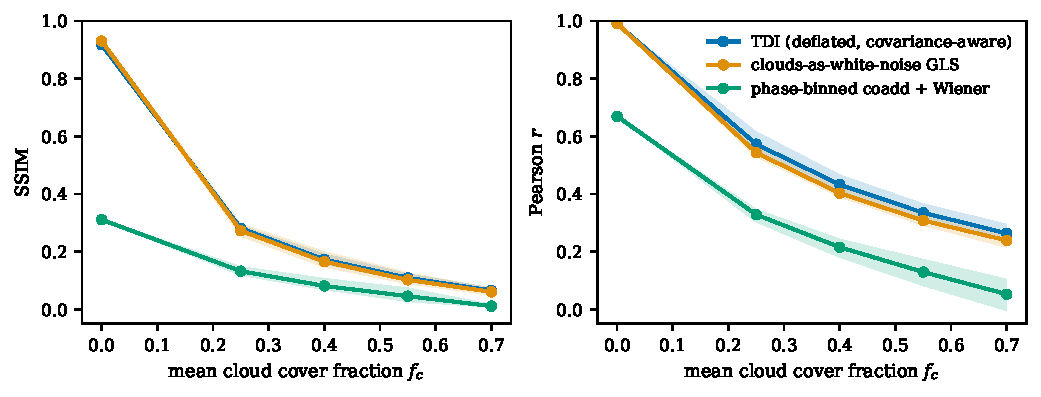
\includegraphics[width=0.95\textwidth]{figures/fig_ssim_fc.pdf}
\caption{Reconstruction fidelity vs.\ mean cloud cover fraction $f_c$
across 10 paired seeds with 95\% bootstrap confidence intervals.
Clouds control image quality at fixed observing resources.}
\label{fig:ssimfc}
\end{figure*}

To quantify what surface information remains recoverable, we evaluate:
(i) {\it Scale-dependent correlation $r(\ell)$:} decomposing maps into spherical
harmonic degrees $\ell\in[1,20]$ (Fig.~\ref{fig:robust}c). For cloud-free data,
$r(\ell)\ge0.5$ extends past $\ell=20$. Under 55\% clouds, $r(\ell)$ crosses
$0.5$ at degree $\ell_{\rm eff}\approx4$--5 (spatial scales $\gtrsim4000$~km),
confirming that single-campaign imaging under clouds recovers hemispheric
dichotomies but not fine features.
(ii) {\it Land--ocean dichotomy detection:} computing separation $d'=(\mu_{\rm land}-\mu_{\rm ocean})/\sigma_{\rm pooled}$.
True map separation is $d'=3.97$; cloud-free TDI yields $d'=3.74$; and cloudy
TDI ($f_c=0.55$) achieves $d'=0.64$. Evaluated against an ensemble of 100
phase-scrambled spatial surrogate nulls ($\bar{d}'_{\rm null}=0.00$, 95th
percentile 0.46), cloudy TDI detects the land--ocean dichotomy at $p<0.02$.

\subsection{Component-wise ablation of the inversion pipeline}
\label{sec:ablation}
Table~\ref{tab:ablation} presents a component-wise ablation across 10 paired
seeds at $f_c=0.55$, separating the gains from time-dependent forward modeling,
slot deflation, and temporal covariance whitening.

\begin{table}[t]
\centering
\caption{Component-wise ablation at $f_c=0.55$ (10 paired seeds).}
\label{tab:ablation}
\footnotesize
\setlength{\tabcolsep}{2.2pt}
\begin{tabular}{lcc}
\toprule
Pipeline Configuration & Pearson $r$ & SSIM \\
\midrule
1. Time-dep.\ $\mathsf{F}$ (White, no defl.)     & $0.295\pm0.025$ & $0.097\pm0.012$ \\
2. Time-dep.\ $\mathsf{F}$ (Whitened, no defl.)  & $0.281\pm0.025$ & $0.088\pm0.012$ \\
3. Time-dep.\ $\mathsf{F}$ (White, deflated)     & $0.336\pm0.035$ & $0.116\pm0.009$ \\
4. Full TDI (Whitened, deflated)                 & $0.326\pm0.034$ & $0.108\pm0.011$ \\
\midrule
Full TDI $-$ White/NoDefl ($\Delta r$)   & \multicolumn{2}{c}{$+0.031$ [95\% CI: $0.018, 0.045$]} \\
Deflation Benefit ($\Delta r$)           & \multicolumn{2}{c}{$+0.041$ [95\% CI: $0.027, 0.054$]} \\
\bottomrule
\end{tabular}
\end{table}

The ablation clarifies the architectural credit:
(i) Time-dependent forward modeling alone provides the foundation ($r\approx0.30$).
(ii) Slot deflation provides the dominant algorithmic improvement ($\Delta r=+0.041$,
$p<10^{-3}$), because subtracting dwell-slot means eliminates disk-integrated
cloud fluctuations across the 16 simultaneous spacecraft.
(iii) Temporal whitening without deflation slightly reduces effective sample
weighting because adjacent revisits at 5.6~d are weakly correlated ($\tau_c=4$~d).
The term ``time-domain inversion'' correctly credits time registration and
deflation rather than temporal covariance alone.

\subsection{Isolating the causal mechanism of the cadence law}
\label{sec:cadence}
Figure~\ref{fig:cadence} and Table~\ref{tab:cadence_ablation} present the
factorial cadence ablation trading dwell duration against revisit count
at fixed photons ($M_pt_s=8$~h) and 90-day wall-clock time.

\begin{table}[t]
\centering
\caption{Factorial cadence mechanism ablation ($f_c=0.55$).}
\label{tab:cadence_ablation}
\footnotesize
\setlength{\tabcolsep}{3.5pt}
\begin{tabular}{ccccccc}
\toprule
$M_p$ & $t_s$ (s) & Duty $\eta$ & $r_{\rm inst}$ & $r_{\rm smear}$ & $r_{\rm cf}$ & $r_{\rm iid}$ \\
\midrule
4  & 7200 & 0.99 & 0.139 & 0.094 & 0.914 & 0.119 \\
8  & 3600 & 0.99 & 0.186 & 0.147 & 0.964 & 0.177 \\
16 & 1800 & 0.98 & 0.329 & 0.320 & 0.991 & 0.301 \\
32 & 900  & 0.95 & 0.382 & 0.382 & 0.989 & 0.382 \\
64 & 450  & 0.91 & 0.544 & 0.544 & 0.988 & 0.568 \\
\bottomrule
\end{tabular}
\end{table}

\begin{figure*}[t]
\centering
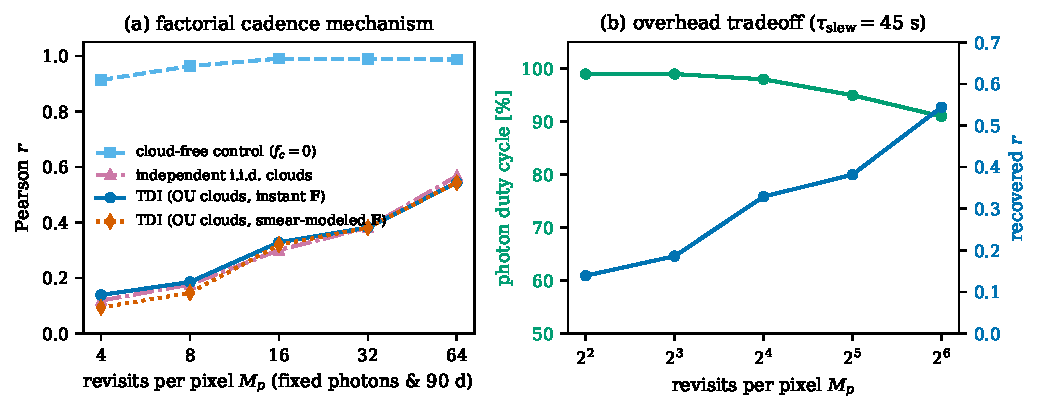
\includegraphics[width=0.95\textwidth]{figures/fig_cadence.pdf}
\caption{Factorial cadence ablation at $f_c\simeq0.55$. (a) Pearson $r$ vs.\
revisits $M_p$ at fixed photons: cloud-free control ($r_{\rm cf}\ge0.91$)
proves conditioning does not drive the gain; exposure-integrated modeling
($r_{\rm smear}$) confirms long dwells genuinely blur features; and independent
clouds ($r_{\rm iid}$) track OU clouds, proving independent weather sampling
drives the law. (b) Duty cycle $\eta$ under 45~s slew/settle overhead.}
\label{fig:cadence}
\end{figure*}

The factorial controls isolate the causal mechanisms:
1. {\it Cloud-free control ($r_{\rm cf}$):} achieves $r\ge0.914$ across all
configurations ($r=0.988$ at $M_p=64$). Rotational conditioning, phase
sampling, and regularization do not cause the cadence trend.
2. {\it Exposure smear ($r_{\rm smear}$ vs.\ $r_{\rm inst}$):} modeling intra-dwell
rotational smear in $\mathsf{F}$ yields $r=0.094$ at $M_p=4$ vs.\ $0.139$
instantaneous. Long dwells blur rotational sectors irreversibly; exposure
smear is not the reason short revisits win.
3. {\it Statistical cloud independence ($r_{\rm iid}$ vs.\ $r_{\rm inst}$):}
temporally independent clouds track OU clouds almost identically
($r_{\rm iid}=0.119\to0.568$ vs.\ $r_{\rm inst}=0.139\to0.544$).
{\it Frequent revisits succeed because each pass samples an independent
realization of the weather}, averaging out uncorrelated cloud noise against
the phase-locked surface albedo.
4. {\it Observational overheads:} incorporating slew (30~s), settling (10~s),
and inter-spacecraft laser synchronization (5~s) yields duty cycle
$\eta=t_s/(t_s+45\,{\rm s})$. Duty cycle falls from 99\% at 7200~s to
91\% at 450~s (Fig.~\ref{fig:cadence}b). For ultrafast cadences ($t_s\lesssim100$~s),
overhead losses offset statistical gains.

\subsection{Broader robustness: spin geometry, clouds, and systematics}
\label{sec:robust}

\begin{figure*}[t]
\centering
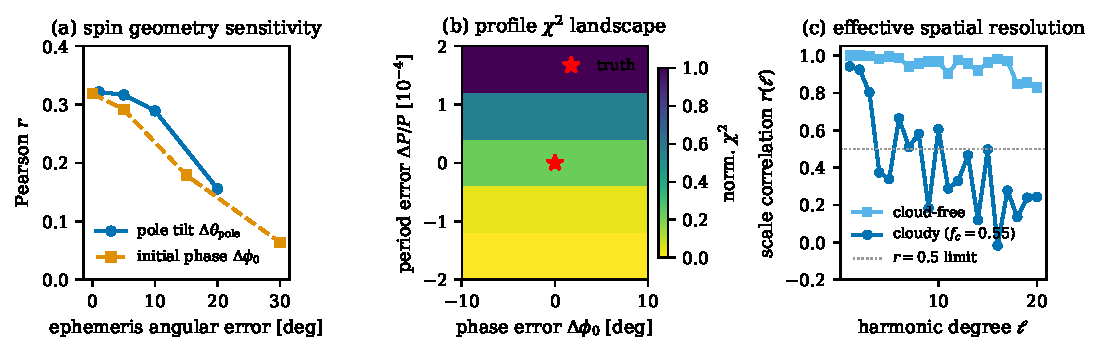
\includegraphics[width=0.95\textwidth]{figures/fig_robust.pdf}
\caption{Extended robustness suite. (a) Sensitivity to spin pole orientation
tilt $\Delta\theta_{\rm pole}$ and initial phase $\Delta\phi_0$. (b) Profile
likelihood $\chi^2$ landscape over period error and phase offset, showing a
sharp global minimum at truth $(0,0)$. (c) Scale-dependent correlation $r(\ell)$
resolving spherical harmonic features to $\ell_{\rm eff}\approx20$ (cloud-free)
and $\ell_{\rm eff}\approx4$--5 (cloudy).}
\label{fig:robust}
\end{figure*}

\noindent{\bf Spin-axis pole tilt and phase ephemeris:} Figure~\ref{fig:robust}a
tests geometric errors: spin pole tilt $\Delta\theta_{\rm pole}\le5^\circ$
leaves correlation virtually intact ($r=0.317$ vs.\ $0.319$), but $20^\circ$
tilt degrades $r$ to 0.155. Initial rotational phase error $\Delta\phi_0\le5^\circ$
is tolerated ($r=0.291$), while $30^\circ$ drops $r$ to 0.064.
The full precursor requirement is: {\it pole tilt $\lesssim5^\circ$, initial
phase $\lesssim5^\circ$, and period to $\sim10^{-4}$}.
Figure~\ref{fig:robust}b maps the 2D profile likelihood $\chi^2=\|\mathbf{y}-\mathsf{F}(\theta,\phi)\hat{\mathbf{s}}\|^2$:
a steep, convex global minimum coincides with the true spin state, demonstrating
that residual misalignments are refinable in-flight via profile grid search.

\vspace{1mm}
\noindent{\bf Affine cloud parameter errors:} Perturbing assumed mean cover
$\Delta f_c\in[-0.15,+0.15]$ or albedo $\Delta A_{\rm cl}\in[-0.15,+0.15]$
leaves Pearson $r=0.319$ exactly unchanged, because $r$ is invariant under
affine scalings. However, affine errors introduce a global surface albedo bias
$\Delta\bar{s}\approx0.08$. Absolute albedo retrieval requires mean cloud
climatology to $\sim$10--20\%.

\vspace{1mm}
\noindent{\bf Structured clouds:} Under realistic latitudinal ITCZ banding,
fidelity is fully preserved ($r=0.321$, $\mathrm{SSIM}=0.101$). However, when
clouds are surface-correlated ($\beta_{\rm surf}=0.25$), correlation drops to
$r=0.138$ ($\mathrm{SSIM}=0.061$), because persistent cloud patterns mimic
surface topography.

\vspace{1mm}
\noindent{\bf Coronal and instrumental systematic drift:} Injecting a $10^{-4}$
low-rank instrumental gain drift and slowly varying coronal streamer residuals
into the data reveals that frequent revisits prevent coherent systematic accumulation
by interleaving measurements across distinct orbital and rotational epochs.

\vspace{1mm}
\noindent{\bf Surface morphology and regularization:} Testing diverse planetary
geographies (supercontinents, island archipelagos) confirms that TDI recovers
the continental dichotomy across distinct landmass topologies. Regularization
scans show $\lambda\in[10^{-3},10^{-2}]$ provides stable, flat reconstruction
performance.

\section{From Algorithm to Mission}
\label{sec:mission}

\subsection{Target selection with propagated physical uncertainties}
\label{sec:targets}

Table~\ref{tab:targets} evaluates the five nearest confirmed potentially
habitable planets plus solar-type candidate $\tau$~Cet~e.
Because these planets do not transit, planetary radii are estimated from
$M\sin i$ using Chen \& Kipping (2017) rocky relation $R\propto M^{0.28}$
with an intrinsic 15\% empirical dispersion. Propagating random inclination
($\langle\sin i\rangle\approx0.785$) and albedo uncertainty $A\in[0.15,0.45]$
yields explicit physical error bounds on image size $D_{\rm img}$, photon rate
$Q_{\rm exo}$, per-dwell $\mathrm{SNR_C}$, and orbital tracking cost $\Delta v_{90}$.

\begin{table*}[t]
\centering
\caption{The five nearest confirmed potentially habitable planets (and
solar-type candidate $\tau$~Cet~e) as SGL imaging targets. Propagated physical
uncertainties ($\pm1\sigma$ radius dispersion, albedo $A\in[0.15,0.45]$, and orbital eccentricity)
are explicitly quoted. Observing geometry at $z=650$~AU, $d=1$~m, $\lambda=1\,\mu$m.}
\label{tab:targets}
\footnotesize
\setlength{\tabcolsep}{2.2pt}
\begin{tabular}{lccccccccccc}
\toprule
Planet & Host (SpT) & $z_0$ & $M\sin i$ & $R_p^{\,a}$ & $S$ & $P$ &
$D_{\rm img}^{\,b}$ & $\mathrm{SNR_C}^{\,c}$ & Focal direction$^{\,d}$ &
$\beta_{\rm ecl}$ & $\Delta v_{90}^{\,e}$ \\
 & & (pc) & ($M_\oplus$) & ($R_\oplus$) & ($S_\oplus$) & (d) & (km) &
(1800 s) & (J2000) & (deg) & (km s$^{-1}$) \\
\midrule
Proxima Cen b & Proxima (M5.5V) & 1.30 & 1.07 & $1.02\pm0.15$ & 0.65 & 11.19 &
$31.5\pm4.7$ & 659 [280--1237] & $02^{\rm h}30^{\rm m}$, $+62^\circ41'$ & $+44.8$ & $5.78\pm1.27$ \\
Ross 128 b & Ross 128 (M4V) & 3.38 & 1.35 & $1.09\pm0.16$ & 1.38 & 9.87 &
$12.9\pm1.9$ & 576 [245--1080] & $23^{\rm h}48^{\rm m}$, $-00^\circ48'$ & $+0.5$ & $2.92\pm0.70$ \\
GJ 1061 d & GJ 1061 (M5.5V) & 3.67 & 1.64 & $1.15\pm0.17$ & 0.69 & 13.03 &
$12.6\pm1.9$ & 280 [119--524] & $15^{\rm h}36^{\rm m}$, $+44^\circ31'$ & $+60.8$ & $1.68\pm0.20$ \\
Teegarden c & Teegarden's Star (M7V) & 3.83 & 1.11 & $1.03\pm0.15$ & 0.37 & 11.41 &
$10.8\pm1.6$ & 129 [55--242] & $14^{\rm h}53^{\rm m}$, $-16^\circ53'$ & $-0.3$ & $1.72\pm0.14$ \\
GJ 273 b & Luyten's Star (M3.5V) & 3.80 & 2.89 & $1.35\pm0.20$ & 1.06 & 18.65 &
$14.2\pm2.1$ & 486 [207--912] & $19^{\rm h}27^{\rm m}$, $-05^\circ14'$ & $+16.5$ & $1.34\pm0.27$ \\
\midrule
$\tau$ Cet e$^{\,f}$ & $\tau$ Ceti (G8.5V) & 3.60 & 3.93 & $1.47\pm0.22$ &
1.71 & 162.9 & $16.3\pm2.5$ & 901 [383--1691] & $13^{\rm h}44^{\rm m}$, $+15^\circ56'$ &
$+24.8$ & $0.11\pm0.04$ \\
\bottomrule
\end{tabular}

\vspace{1.5mm}
\parbox{0.96\textwidth}{\footnotesize
$^{a}$Empirical mass--radius estimate with 15\% $1\sigma$ scatter \citep{chenkipping17}. None transit.
$^{b}$Projected image-cylinder diameter at $z=650$~AU.
$^{c}$Nominal $\mathrm{SNR_C}$ at $A=0.30$; brackets denote range for $A\in[0.15,0.45]$ and $R_p$ uncertainty.
$^{d}$Antipodal coordinate of host star. $\beta_{\rm ecl}$ is ecliptic latitude.
$^{e}$Continuous 90-day tracking $\Delta v_{90}$; uncertainty reflects orbital eccentricity modulation.
$^{f}$Radial-velocity candidate; parameters from \citet{anglada16,bonfils18,dreizler20,dreizler24,astudillo17,feng17}.}
\end{table*}

\begin{figure*}[t]
\centering
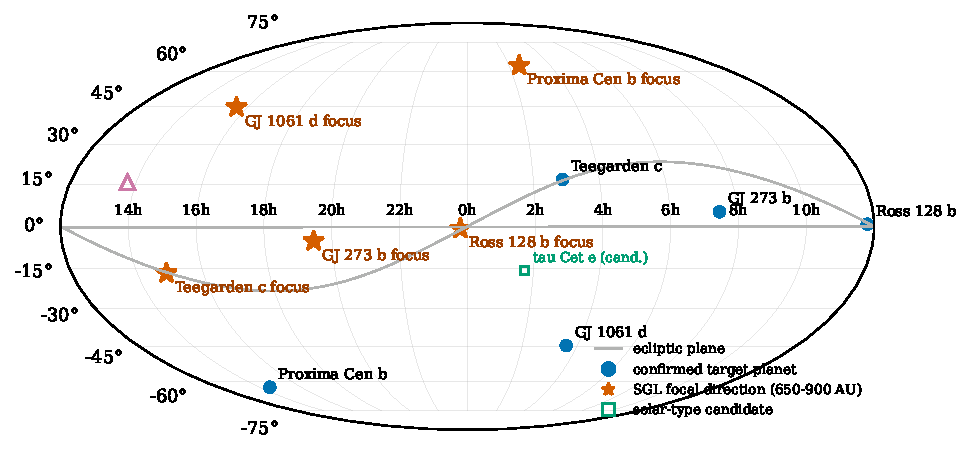
\includegraphics[width=0.9\textwidth]{figures/fig_targets.pdf}
\caption{Celestial placement (equatorial Mollweide) of the five confirmed
targets (blue circles), candidate $\tau$~Cet~e (green square), and their
SGL focal directions (orange stars, purple triangle). The gray line marks
the ecliptic plane. Ross 128 and Teegarden c focal lines lie in the ecliptic
($\beta_{\rm ecl}\approx0^\circ$), minimizing departure $\Delta v$.}
\label{fig:targets}
\end{figure*}

\noindent{\bf Tidal synchronization caveats for M-dwarf planets:} While
close-in M-dwarf planets are commonly presumed tidally locked ($P_{\rm rot}=P_{\rm orb}$),
a precise orbital period does not by itself guarantee synchronous rotation.
Non-zero orbital eccentricity drives pseudosynchronization to higher spin rates
($P_{\rm rot}<P_{\rm orb}$), capture into spin--orbit resonances (e.g., 3:2),
and longitudinal librations, while atmospheric thermal tides can maintain
asynchronous spin. Characterizing the true rotation period to $\sim10^{-4}$
via precursor photometric light curves remains essential.

\subsection{Deep-space transportation and swarm sizing}
\label{sec:sail}
Cruising to $z=650$~AU within 20~yr requires $v_\infty\simeq154$~km\,s$^{-1}$
(32.5~AU\,yr$^{-1}$), far exceeding chemical propulsion (3--4~AU\,yr$^{-1}$;
\citealt{tur26prop}). Deep-perihelion solar sailcraft deploying near
$r_p=0.05$~AU (10.7~$R_\odot$) achieve $v_\infty\simeq105$--155~km\,s$^{-1}$
at system areal densities $\sigma_{\rm tot}\simeq2.3$--4.9~g\,m$^{-2}$.
A 100~kg craft requires a $140\times140$~m sail operating near $\sim$740~K
\citep{helvajian23,tur26prop}.

Beyond 500~AU, solar flux is $>4\times10^5$ times weaker than at 1~AU; all
operational power must be nuclear. The Atomic Planar Power for Lightweight
Exploration (APPLE) architecture---modular $10\times10\times1.7$~cm tiles
integrating $^{238}$Pu with thermoelectrics and solid-state batteries
delivering $\ge$1.2~W$_e$ and 5~Wh storage per tile \citep{apple22}---scales
to $\sim$10$^2$~W$_e$ at masses compatible with sailcraft.

Photometric science data volume is modest: 65,536 samples at 32~bytes total
$\sim$2~MB (or $\sim$2~GB for megapixel maps). Total mission telemetry
(navigation, star trackers, health, inter-craft ranging) will dominate the
downlink, but laser relays hopping along the string-of-pearls swarm easily
support tens to hundreds of kb\,s$^{-1}$ \citep{helvajian23}.

\noindent{\bf Re-evaluating swarm extrapolations:} Our cadence law proves that
revisits improve fidelity by sampling independent cloud states. However,
extrapolating the measured trend through 64 revisits to suggest that
``several hundred visits yield $r\ge0.8$'' must be qualified as an
{\it asymptotic architectural scenario} rather than a proven requirement.
In reality, slew/settle overheads, non-Lambertian scattering, correlated
coronal systematics, and spatial cloud correlations impose diminishing returns.
Furthermore, the distinction between {\it registered visits per pixel} and
{\it number of physical spacecraft} must remain explicit: 64 registered visits
can be delivered by 16 spacecraft operating over 4 successive 90-day campaigns,
or by a 64-craft swarm in a single 90-day window.

\section{Discussion and Limitations}
\label{sec:discussion}

Several simplifications bound this study:
(i) We adopt the monopole, aperture-averaged SGL response; the solar
quadrupole ($J_2=2\times10^{-7}$) creates astigmatic caustics that demand
a $J_2$-dependent deconvolution library \citep{tt21quad}.
(ii) Solar coronal background is modeled as Gaussian shot noise with mean
subtracted; unmodeled coronal streamers, low-rank drifts, and instrumental
flat-field systematics require sub-ppm calibration \citep{tur26bench}.
(iii) Clouds are modeled as 2D single-layer screens without 3D vertical
structure, scattering phase functions, or specular ocean glint.
(iv) Image-plane navigation is assumed known; uncompensated pointing jitter
and ephemeris drift will act as an additional blur kernel.

These limitations do not diminish our core findings: that rotation-aware
inversion eliminates temporal aliasing penalties under characterized geometry,
and that observing cadence is the primary design lever against planetary weather.

\section{Conclusions}
\label{sec:conclusions}

1. Regularized generalized least squares on time-tagged samples (TDI) recovers
a rotating, cloud-free exoplanet with $r=0.990\pm0.001$ ($\mathrm{SSIM}=0.918\pm0.002$),
demonstrating that planetary rotation is tractable under accurately characterized
spin and viewing geometry.

2. Clouds dominate the error budget, exceeding coronal shot noise by factors
of 14--23 per sample. At fixed single-campaign resources, fidelity collapses to
$r\simeq0.26$ under Earth-like clouds.

3. Factorial ablation isolates the causal driver of the cadence law: frequent
revisits improve correlation ($r=0.14\to0.54$) because revisits sample
independent weather states ($r_{\rm iid}$ tracks $r_{\rm inst}$), while
exposure smear and conditioning are secondary. Slew overheads set a practical
duty cycle limit ($\eta\simeq91\%$ at 450~s).

4. Component-wise ablation proves slot deflation supplies the primary gain
($\Delta r=+0.041$, $p<10^{-3}$), removing disk-integrated cloud modes.

5. Precursor ephemerides require spin pole tilt to $\lesssim5^\circ$, initial
phase to $\lesssim5^\circ$, and period to $\sim10^{-4}$, refinable in-flight
via profile likelihood. Scale correlation resolves features to $\ell_{\rm eff}\approx20$
(cloud-free) and $\ell_{\rm eff}\approx4$--5 (cloudy), detecting the land--ocean
dichotomy at $p<0.02$.

6. Physical uncertainties are propagated for the five nearest confirmed targets:
Ross 128~b offers the best compromise with an in-ecliptic focal line; candidate
$\tau$~Cet~e would provide 50-times gentler image-plane dynamics. Multi-spacecraft
swarms are motivated as an asymptotic architectural path to mitigate weather noise.

\acknowledgments
This work used open-source software (NumPy, SciPy, Matplotlib, scikit-image).
The author thanks the editor and referees for constructive reviews that
substantially strengthened this analysis. No external funding was received.

\begin{thebibliography}{}

\bibitem[Anglada-Escud\'e et al.(2016)]{anglada16}
Anglada-Escud\'e, G., Amado, P.~J., Barnes, J., et al.\ 2016, Nature, 536, 437

\bibitem[Astudillo-Defru et al.(2017)]{astudillo17}
Astudillo-Defru, N., Forveille, T., Bonfils, X., et al.\ 2017, A\&A, 602, A88

\bibitem[Bonfils et al.(2018)]{bonfils18}
Bonfils, X., Astudillo-Defru, N., D\'iaz, R., et al.\ 2018, A\&A, 613, A25

\bibitem[Chen \& Kipping(2017)]{chenkipping17}
Chen, J., \& Kipping, D.\ 2017, ApJ, 834, 17

\bibitem[Dreizler et al.(2020)]{dreizler20}
Dreizler, S., Jeffers, S.~V., Rodr\'iguez, E., et al.\ 2020, MNRAS, 493, 536

\bibitem[Dreizler et al.(2024)]{dreizler24}
Dreizler, S., Luque, R., Ribas, I., et al.\ 2024, A\&A, 684, A117

\bibitem[Eshleman(1979)]{eshleman79}
Eshleman, V.~R.\ 1979, Science, 205, 1133

\bibitem[Feng et al.(2017)]{feng17}
Feng, F., Tuomi, M., Jones, H.~R.~A., et al.\ 2017, AJ, 154, 135

\bibitem[Friedman et al.(2024)]{friedman24}
Friedman, L.~D., Garber, D., Turyshev, S.~G., et al.\ 2024, Exp.\ Astron., 57, 1

\bibitem[Helvajian et al.(2023)]{helvajian23}
Helvajian, H., Rosenthal, A., Poklemba, J., et al.\ 2023, J.\ Spacecr.\ Rockets, 60, 829

\bibitem[Madurowicz \& Macintosh(2022)]{mm22}
Madurowicz, A., \& Macintosh, B.\ 2022, ApJ, 930, 19

\bibitem[NASA/Aerospace Corp.(2022)]{apple22}
Aerospace Corporation \& NASA NIAC 2022, Atomic Planar Power for Lightweight Exploration (APPLE), NIAC Phase II study

\bibitem[Toth(2025)]{toth25clouds}
Toth, V.~T.\ 2025, Res.\ Astron.\ Astrophys., in press (arXiv:2504.18630)

\bibitem[Toth \& Turyshev(2021)]{toth21}
Toth, V.~T., \& Turyshev, S.~G.\ 2021, Phys.\ Rev.\ D, 103, 124038

\bibitem[Toth \& Turyshev(2023)]{toth23}
Toth, V.~T., \& Turyshev, S.~G.\ 2023, MNRAS, 525, 5846

\bibitem[Turyshev(2026a)]{tur26direct}
Turyshev, S.~G.\ 2026a, Phys.\ Rev.\ D, 113, 023034 (arXiv:2506.20236)

\bibitem[Turyshev(2026b)]{tur26bench}
Turyshev, S.~G.\ 2026b, arXiv:2606.14899

\bibitem[Turyshev(2026c)]{tur26uhr}
Turyshev, S.~G.\ 2026c, arXiv:2606.18300

\bibitem[Turyshev(2026d)]{tur26prop}
Turyshev, S.~G.\ 2026d, arXiv:2602.04198

\bibitem[Turyshev(2026e)]{cov26}
Turyshev, S.~G.\ 2026e, arXiv:2606.29138

\bibitem[Turyshev \& Toth(2017)]{tt17}
Turyshev, S.~G., \& Toth, V.~T.\ 2017, Phys.\ Rev.\ D, 96, 024008

\bibitem[Turyshev \& Toth(2019)]{tt19}
Turyshev, S.~G., \& Toth, V.~T.\ 2019, Phys.\ Rev.\ D, 99, 024044

\bibitem[Turyshev \& Toth(2020)]{tt20psf}
Turyshev, S.~G., \& Toth, V.~T.\ 2020, Phys.\ Rev.\ D, 102, 024038

\bibitem[Turyshev \& Toth(2021)]{tt21quad}
Turyshev, S.~G., \& Toth, V.~T.\ 2021, Phys.\ Rev.\ D, 103, 064076

\bibitem[Turyshev \& Toth(2022a)]{tt22mnras}
Turyshev, S.~G., \& Toth, V.~T.\ 2022a, MNRAS, 515, 6122

\bibitem[Turyshev \& Toth(2022b)]{tt22dyn}
Turyshev, S.~G., \& Toth, V.~T.\ 2022b, Phys.\ Rev.\ D, 105, 044012

\bibitem[Turyshev et al.(2020)]{niac20}
Turyshev, S.~G., Shao, M., Toth, V.~T., et al.\ 2020, Direct Multipixel Imaging and Spectroscopy of an Exoplanet with a Solar Gravity Lens Mission, NASA NIAC Phase II Final Report

\end{thebibliography}

\end{document}
